\documentclass[12pt,letterpaper]{article}\usepackage[]{graphicx}\usepackage[]{color}
%% maxwidth is the original width if it is less than linewidth
%% otherwise use linewidth (to make sure the graphics do not exceed the margin)
\makeatletter
\def\maxwidth{ %
  \ifdim\Gin@nat@width>\linewidth
    \linewidth
  \else
    \Gin@nat@width
  \fi
}
\makeatother

\definecolor{fgcolor}{rgb}{0.345, 0.345, 0.345}
\newcommand{\hlnum}[1]{\textcolor[rgb]{0.686,0.059,0.569}{#1}}%
\newcommand{\hlstr}[1]{\textcolor[rgb]{0.192,0.494,0.8}{#1}}%
\newcommand{\hlcom}[1]{\textcolor[rgb]{0.678,0.584,0.686}{\textit{#1}}}%
\newcommand{\hlopt}[1]{\textcolor[rgb]{0,0,0}{#1}}%
\newcommand{\hlstd}[1]{\textcolor[rgb]{0.345,0.345,0.345}{#1}}%
\newcommand{\hlkwa}[1]{\textcolor[rgb]{0.161,0.373,0.58}{\textbf{#1}}}%
\newcommand{\hlkwb}[1]{\textcolor[rgb]{0.69,0.353,0.396}{#1}}%
\newcommand{\hlkwc}[1]{\textcolor[rgb]{0.333,0.667,0.333}{#1}}%
\newcommand{\hlkwd}[1]{\textcolor[rgb]{0.737,0.353,0.396}{\textbf{#1}}}%

\usepackage{framed}
\makeatletter
\newenvironment{kframe}{%
 \def\at@end@of@kframe{}%
 \ifinner\ifhmode%
  \def\at@end@of@kframe{\end{minipage}}%
  \begin{minipage}{\columnwidth}%
 \fi\fi%
 \def\FrameCommand##1{\hskip\@totalleftmargin \hskip-\fboxsep
 \colorbox{shadecolor}{##1}\hskip-\fboxsep
     % There is no \\@totalrightmargin, so:
     \hskip-\linewidth \hskip-\@totalleftmargin \hskip\columnwidth}%
 \MakeFramed {\advance\hsize-\width
   \@totalleftmargin\z@ \linewidth\hsize
   \@setminipage}}%
 {\par\unskip\endMakeFramed%
 \at@end@of@kframe}
\makeatother

\definecolor{shadecolor}{rgb}{.97, .97, .97}
\definecolor{messagecolor}{rgb}{0, 0, 0}
\definecolor{warningcolor}{rgb}{1, 0, 1}
\definecolor{errorcolor}{rgb}{1, 0, 0}
\newenvironment{knitrout}{}{} % an empty environment to be redefined in TeX

\usepackage{alltt}
 \usepackage[left=2cm,right=2cm,top=2cm,bottom=2cm]{geometry}
\usepackage[ansinew]{inputenc}
\usepackage[spanish]{babel}
\usepackage{amsmath}
\usepackage{amsfonts}
\usepackage{amssymb}
\usepackage{dsfont}
\usepackage{multicol} 
\usepackage{subfigure}
\usepackage{graphicx}
\usepackage{float} 
\usepackage{verbatim} 
\usepackage[left=2cm,right=2cm,top=2cm,bottom=2cm]{geometry}
\usepackage{fancyhdr}
\pagestyle{fancy} 
\fancyhead[LO]{\leftmark}
\usepackage{caption}
\newtheorem{definicion}{Definci\'on}
\IfFileExists{upquote.sty}{\usepackage{upquote}}{}
\begin{document}

\begin{titlepage}
\setlength{\unitlength}{1 cm} %Especificar unidad de trabajo

\begin{center}
\textbf{{\large UNIVERSIDAD DE EL SALVADOR}\\
{\large FACULTAD MULTIDISCIPLINARIA DE OCCIDENTE}\\
{\large DEPARTAMENTO DE MATEM\'ATICA}}\\ [0.50 cm]

\begin{picture}(18,4)
 \put(7,0){
\includegraphics[width=4cm]{minerva.jpg}}
\end{picture}
\\[0.25 cm]

\textbf{{\large Licenciatura en Estad\'istica}\\ [1.25cm]
{\large Control Estad\'istico del Paquete R }\\ [2 cm]
%\setlength{\unitlength}{1 cm}
{\large  \textbf{''UNIDAD DOS"}}\\ [3 cm]
{\large Alumna:}\\
{\large Erika Beatr\'iz Guill\'en Pineda}\\ [2cm]
{\large Fecha de elaboraci\'on}\\
Santa Ana - \today }
\end{center}
\end{titlepage}

\newtheorem{teorema}{Teorema}
\newtheorem{prop}{Proposici\'on}[section]

\lhead{Pr\'actica 07}

\lfoot{LICENCIATURA EN ESTAD\'ISTICA}
\cfoot{UESOCC}
\rfoot{\thepage}
%\pagestyle{fancy} 

\setcounter{page}{1}
\newpage

\section {AN\'ALISIS ESTAD\'ISTICO DE LOS DATOS}

\begin {itemize}
\item Ejemplo:
\end{itemize}

\begin {itemize}
\item 1) Activar el directorio de trabajo
\begin{knitrout}
\definecolor{shadecolor}{rgb}{0.969, 0.969, 0.969}\color{fgcolor}\begin{kframe}
\begin{alltt}
\hlkwd{getwd}\hlstd{()}
\end{alltt}
\begin{verbatim}
## [1] "C:/Users/User/Documents/TODAS_PRACTICAS"
\end{verbatim}
\begin{alltt}
\hlkwd{setwd}\hlstd{(}\hlstr{"C:/Users/User/Documents/TODAS_PRACTICAS"}\hlstd{)}
\end{alltt}
\end{kframe}
\end{knitrout}
\item 2) Crear un nuevo Script y llamarle "Script07-DatosDiscretos"

\item 3) Crear el vector de datos
\begin{knitrout}
\definecolor{shadecolor}{rgb}{0.969, 0.969, 0.969}\color{fgcolor}\begin{kframe}
\begin{alltt}
\hlstd{Hijos} \hlkwb{<-} \hlkwd{c}\hlstd{(}\hlnum{2}\hlstd{,} \hlnum{1}\hlstd{,} \hlnum{2}\hlstd{,} \hlnum{1}\hlstd{,} \hlnum{4}\hlstd{,} \hlnum{2}\hlstd{,} \hlnum{3}\hlstd{,} \hlnum{0}\hlstd{,} \hlnum{2}\hlstd{,} \hlnum{3}\hlstd{,} \hlnum{3}\hlstd{,} \hlnum{2}\hlstd{,} \hlnum{1}\hlstd{,} \hlnum{0}\hlstd{,} \hlnum{2}\hlstd{,} \hlnum{4}\hlstd{,} \hlnum{1}\hlstd{,} \hlnum{2}\hlstd{,}
           \hlnum{1}\hlstd{,} \hlnum{3}\hlstd{,} \hlnum{4}\hlstd{,} \hlnum{1}\hlstd{,} \hlnum{2}\hlstd{,} \hlnum{3}\hlstd{,} \hlnum{1}\hlstd{,} \hlnum{5}\hlstd{,} \hlnum{2}\hlstd{,} \hlnum{3}\hlstd{,} \hlnum{1}\hlstd{,} \hlnum{2}\hlstd{)}
\hlkwd{data.entry}\hlstd{(Hijos)}
\hlstd{Hijos}
\end{alltt}
\begin{verbatim}
##  [1] 2 1 2 1 4 2 3 0 2 3 3 2 1 0 2 4 1 2 1 3 4 1 2 3 1 5 2 3 1 2
\end{verbatim}
\begin{alltt}
\hlkwd{length}\hlstd{(Hijos)}
\end{alltt}
\begin{verbatim}
## [1] 30
\end{verbatim}
\end{kframe}
\end{knitrout}
\item 4) Guardar el vector de datos en un archivo de texto
\begin{knitrout}
\definecolor{shadecolor}{rgb}{0.969, 0.969, 0.969}\color{fgcolor}\begin{kframe}
\begin{alltt}
\hlkwd{write}\hlstd{(Hijos,} \hlstr{"Hijos.txt"}\hlstd{)}
\end{alltt}
\end{kframe}
\end{knitrout}
\item 5) Limpiar el ?rea de trabajo (Workspace)
\begin{knitrout}
\definecolor{shadecolor}{rgb}{0.969, 0.969, 0.969}\color{fgcolor}\begin{kframe}
\begin{alltt}
\hlkwd{ls}\hlstd{()}
\end{alltt}
\begin{verbatim}
## [1] "Hijos"
\end{verbatim}
\begin{alltt}
\hlkwd{rm}\hlstd{(}\hlkwc{list}\hlstd{=}\hlkwd{ls}\hlstd{(}\hlkwc{all}\hlstd{=}\hlnum{TRUE}\hlstd{));}
\hlkwd{ls}\hlstd{()}
\end{alltt}
\begin{verbatim}
## character(0)
\end{verbatim}
\end{kframe}
\end{knitrout}
\newpage
\item 6) Leer o recuperar el vector de datos o archivo de texto
\begin{knitrout}
\definecolor{shadecolor}{rgb}{0.969, 0.969, 0.969}\color{fgcolor}\begin{kframe}
\begin{alltt}
\hlstd{X} \hlkwb{<-} \hlkwd{scan}\hlstd{(}\hlstr{"Hijos.txt"}\hlstd{,} \hlkwc{what} \hlstd{=} \hlkwd{integer}\hlstd{(}\hlnum{0}\hlstd{),} \hlkwc{na.strings} \hlstd{=} \hlstr{"NA"}\hlstd{,} \hlkwc{flush}\hlstd{=}\hlnum{FALSE}\hlstd{)}
\hlkwd{ls}\hlstd{()}
\end{alltt}
\begin{verbatim}
## [1] "X"
\end{verbatim}
\begin{alltt}
\hlcom{# Si el vector contiene caracteres se usa: what = character()}
\hlcom{# Si el vector contiene reales se ocupa: what = double(0)}
\end{alltt}
\end{kframe}
\end{knitrout}
\item 7) Elaborar el gr\'afico de puntos y diagrama de tallo-hojas (stem-and-leaf)
\begin{knitrout}
\definecolor{shadecolor}{rgb}{0.969, 0.969, 0.969}\color{fgcolor}\begin{kframe}
\begin{alltt}
\hlcom{# Gr?fico de puntos}
\hlkwd{stripchart}\hlstd{(X,} \hlkwc{method}\hlstd{=}\hlstr{"stack"}\hlstd{,} \hlkwc{vertical}\hlstd{=}\hlnum{FALSE}\hlstd{,} \hlkwc{col}\hlstd{=}\hlstr{"blue"}\hlstd{,} \hlkwc{pch}\hlstd{=}\hlnum{1}\hlstd{,} \hlkwc{main}\hlstd{=}\hlstr{"Gr\textbackslash{}'afico de\textbackslash{}n
puntos"}\hlstd{,} \hlkwc{xlab}\hlstd{=}\hlstr{"N\textbackslash{}'umero de hijos"}\hlstd{)}
\end{alltt}
\end{kframe}
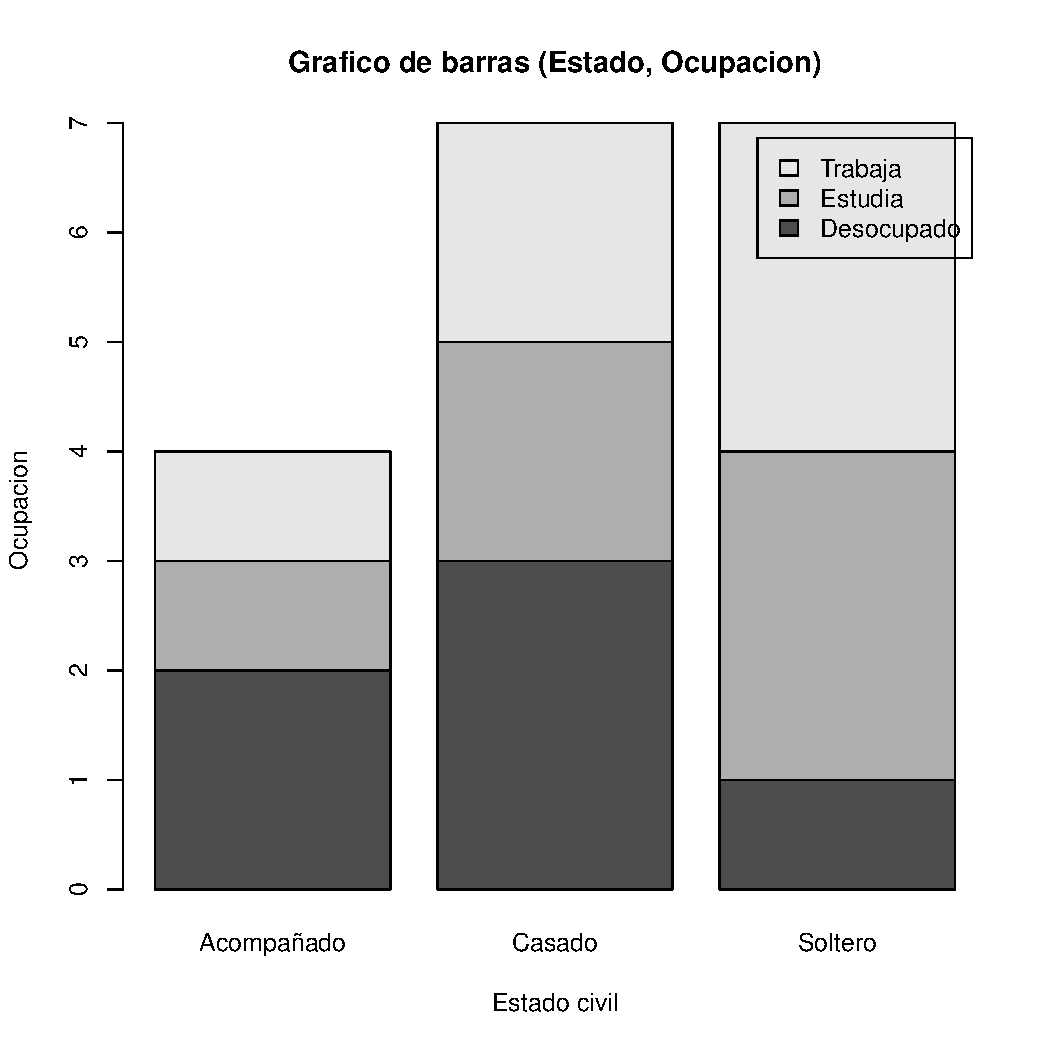
\includegraphics[width=\maxwidth]{figure/unnamed-chunk-6-1} 
\begin{kframe}\begin{alltt}
\hlcom{# Observaci\textbackslash{}'on: method puede ser:}
\hlcom{# "overplot" (los puntos coincidentes son superpuestos)}
\hlcom{# "jitter" (los puntos se ven como alejados o inquietos)}
\hlcom{# "stack" (los puntos coincidentes son apilados, uno tras otro)}
\end{alltt}
\end{kframe}
\end{knitrout}
\item 8) Crear la tabla de frecuencias completa
\begin{knitrout}
\definecolor{shadecolor}{rgb}{0.969, 0.969, 0.969}\color{fgcolor}\begin{kframe}
\begin{alltt}
\hlcom{# Frecuencias individuales}
\hlstd{fab} \hlkwb{<-} \hlkwd{table}\hlstd{(X); fab} \hlcom{# Frecuencias absolutas}
\end{alltt}
\begin{verbatim}
## X
##  0  1  2  3  4  5 
##  2  8 10  6  3  1
\end{verbatim}
\begin{alltt}
\hlstd{fre} \hlkwb{<-} \hlstd{fab}\hlopt{/}\hlkwd{length}\hlstd{(X); fre} \hlcom{# Frecuencias relativas}
\end{alltt}
\begin{verbatim}
## X
##          0          1          2          3          4          5 
## 0.06666667 0.26666667 0.33333333 0.20000000 0.10000000 0.03333333
\end{verbatim}
\begin{alltt}
\hlstd{Fac} \hlkwb{<-} \hlkwd{cumsum}\hlstd{(fab); Fac} \hlcom{# Frecuencias acumuladas}
\end{alltt}
\begin{verbatim}
##  0  1  2  3  4  5 
##  2 10 20 26 29 30
\end{verbatim}
\begin{alltt}
\hlstd{Far} \hlkwb{<-} \hlstd{Fac}\hlopt{/}\hlkwd{length}\hlstd{(X); Far} \hlcom{# Frecuencias acumuladas relativas}
\end{alltt}
\begin{verbatim}
##          0          1          2          3          4          5 
## 0.06666667 0.33333333 0.66666667 0.86666667 0.96666667 1.00000000
\end{verbatim}
\begin{alltt}
\hlcom{# Tabla de frecuencias completa}
\hlkwd{options}\hlstd{(}\hlkwc{digits}\hlstd{=}\hlnum{2}\hlstd{)}
\hlstd{tabla} \hlkwb{<-} \hlkwd{data.frame}\hlstd{(}\hlkwc{fab}\hlstd{=fab,} \hlkwc{fre}\hlstd{=fre,} \hlkwc{Fac}\hlstd{=Fac,} \hlkwc{Far}\hlstd{=Far)}
\hlkwd{names}\hlstd{(tabla)} \hlkwb{<-} \hlkwd{c}\hlstd{(}\hlstr{"X"}\hlstd{,} \hlstr{"fab"}\hlstd{,} \hlstr{"free.X"}\hlstd{,} \hlstr{"fre"}\hlstd{,} \hlstr{"Fac"}\hlstd{,} \hlstr{"Far"}\hlstd{)}
\hlstd{tabla}
\end{alltt}
\begin{verbatim}
##   X fab free.X   fre Fac   Far
## 0 0   2      0 0.067   2 0.067
## 1 1   8      1 0.267  10 0.333
## 2 2  10      2 0.333  20 0.667
## 3 3   6      3 0.200  26 0.867
## 4 4   3      4 0.100  29 0.967
## 5 5   1      5 0.033  30 1.000
\end{verbatim}
\begin{alltt}
\hlstd{tfre} \hlkwb{<-} \hlkwd{data.frame}\hlstd{(}\hlkwc{X}\hlstd{=tabla}\hlopt{$}\hlstd{X,} \hlkwc{fab}\hlstd{=tabla}\hlopt{$}\hlstd{fab,} \hlkwc{fre}\hlstd{=tabla}\hlopt{$}\hlstd{fre,}
                   \hlkwc{Fac}\hlstd{=tabla}\hlopt{$}\hlstd{Fac,} \hlkwc{Far}\hlstd{=tabla}\hlopt{$}\hlstd{Far)}
\hlstd{tfre}
\end{alltt}
\begin{verbatim}
##   X fab   fre Fac   Far
## 1 0   2 0.067   2 0.067
## 2 1   8 0.267  10 0.333
## 3 2  10 0.333  20 0.667
## 4 3   6 0.200  26 0.867
## 5 4   3 0.100  29 0.967
## 6 5   1 0.033  30 1.000
\end{verbatim}
\begin{alltt}
\hlcom{# Note que el cuadro resultante no tiene la presentaci\textbackslash{}'on deseada para }
\hlcom{# presentarla en un informe. Sin embargo, si estamos utilizando LATEX }
\hlcom{# podemos utilizar la siguiente instrucci\textbackslash{}'on xtable(tfre) y con esto nos }
\hlcom{# genera el c\textbackslash{}'odigo correspondiente para incorporarlo en nuestro archivo.}
\end{alltt}
\end{kframe}
\end{knitrout}
\item 9) Calcular los estad?sticos descriptivos de la variable
\begin{knitrout}
\definecolor{shadecolor}{rgb}{0.969, 0.969, 0.969}\color{fgcolor}\begin{kframe}
\begin{alltt}
\hlcom{# Estad?sticos de tendencia central de los datos}
\hlstd{media} \hlkwb{<-} \hlkwd{mean}\hlstd{(X,} \hlkwc{na.rm} \hlstd{=} \hlnum{FALSE}\hlstd{);}
\hlstd{media}
\end{alltt}
\begin{verbatim}
## [1] 2.1
\end{verbatim}
\begin{alltt}
\hlcom{# na.rm = FALSE, le indica a R que los datos faltantes son omitidos }
\hlcom{# en el c?lculo de la media.}
\hlkwa{for}\hlstd{(i} \hlkwa{in} \hlnum{1}\hlopt{:}\hlkwd{length}\hlstd{(X))} \hlkwa{if} \hlstd{(fab[i]} \hlopt{==} \hlkwd{max}\hlstd{(fab))} \hlkwa{break}\hlstd{()}
\hlstd{moda} \hlkwb{<-} \hlkwd{names}\hlstd{(fab[i]);}
\hlstd{moda} \hlcom{# R no tiene incorporada una funci\textbackslash{}'on para la moda}
\end{alltt}
\begin{verbatim}
## [1] "2"
\end{verbatim}
\begin{alltt}
\hlstd{mediana} \hlkwb{<-} \hlkwd{median}\hlstd{(X);}
\hlstd{mediana}
\end{alltt}
\begin{verbatim}
## [1] 2
\end{verbatim}
\begin{alltt}
\hlcom{# Estad\textbackslash{}'isticos de dispersi\textbackslash{}'on o variabilidad de los datos}
\hlkwd{range}\hlstd{(X)} \hlcom{# Devuelve el valor m\textbackslash{}'inimo y m\textbackslash{}'aximo del conjunto de datos.}
\end{alltt}
\begin{verbatim}
## [1] 0 5
\end{verbatim}
\begin{alltt}
\hlstd{cuasivar} \hlkwb{<-} \hlkwd{var}\hlstd{(X);}
\hlstd{cuasivar}
\end{alltt}
\begin{verbatim}
## [1] 1.5
\end{verbatim}
\begin{alltt}
\hlstd{s} \hlkwb{<-} \hlkwd{sd}\hlstd{(X);}
\hlstd{s}
\end{alltt}
\begin{verbatim}
## [1] 1.2
\end{verbatim}
\begin{alltt}
\hlcom{# Devuelve la cuasivarianza y la cuasivarianza muestral}
\hlkwd{quantile}\hlstd{(X,}\hlkwd{c}\hlstd{(}\hlnum{0.25}\hlstd{,} \hlnum{0.5}\hlstd{,} \hlnum{0.75}\hlstd{))}
\end{alltt}
\begin{verbatim}
## 25% 50% 75% 
##   1   2   3
\end{verbatim}
\begin{alltt}
\hlcom{# C?lculo de Q1, Q2, Q3}
\hlkwd{quantile}\hlstd{(X,} \hlnum{0.6}\hlstd{)}
\end{alltt}
\begin{verbatim}
## 60% 
##   2
\end{verbatim}
\begin{alltt}
\hlcom{# En general se pueden encontrar cualquier percentil}
\hlcom{# Conocer un resumen de los datos}
\hlstd{resumen} \hlkwb{<-} \hlkwd{summary}\hlstd{(X);}
\hlstd{resumen}
\end{alltt}
\begin{verbatim}
##    Min. 1st Qu.  Median    Mean 3rd Qu.    Max. 
##     0.0     1.0     2.0     2.1     3.0     5.0
\end{verbatim}
\begin{alltt}
\hlcom{# Min, Q1, Median, Mean, Q3, Max}
\hlkwd{fivenum}\hlstd{(X)}
\end{alltt}
\begin{verbatim}
## [1] 0 1 2 3 5
\end{verbatim}
\begin{alltt}
\hlcom{# min, cuartil menor, mediana, cuartil mayor, max}
\end{alltt}
\end{kframe}
\end{knitrout}
\item 10) Elaborar los gr\'aficos que se le pueden aplicar a la variable discreta
\begin{knitrout}
\definecolor{shadecolor}{rgb}{0.969, 0.969, 0.969}\color{fgcolor}\begin{kframe}
\begin{alltt}
\hlcom{# Gr?fico de barras (por ser pocos valores)}
\hlkwd{barplot}\hlstd{(tfre[[}\hlnum{2}\hlstd{]],} \hlkwc{main}\hlstd{=}\hlstr{"Gr?fico de barras"}\hlstd{,} \hlkwc{xlab}\hlstd{=}\hlstr{"X = N?mero Hijos\textbackslash{}n"}\hlstd{,}
        \hlkwc{ylab}\hlstd{=}\hlstr{"frecuencia"}\hlstd{,}\hlkwc{col}\hlstd{=}\hlkwd{c}\hlstd{(}\hlstr{"yellow"}\hlstd{,} \hlstr{"blue"}\hlstd{,} \hlstr{"white"}\hlstd{,} \hlstr{"orange"}\hlstd{,}
                                \hlstr{"cyan"}\hlstd{,} \hlstr{"red"}\hlstd{),} \hlkwc{sub}\hlstd{=}\hlstr{"Agosto-2012"}\hlstd{)}
\end{alltt}
\end{kframe}
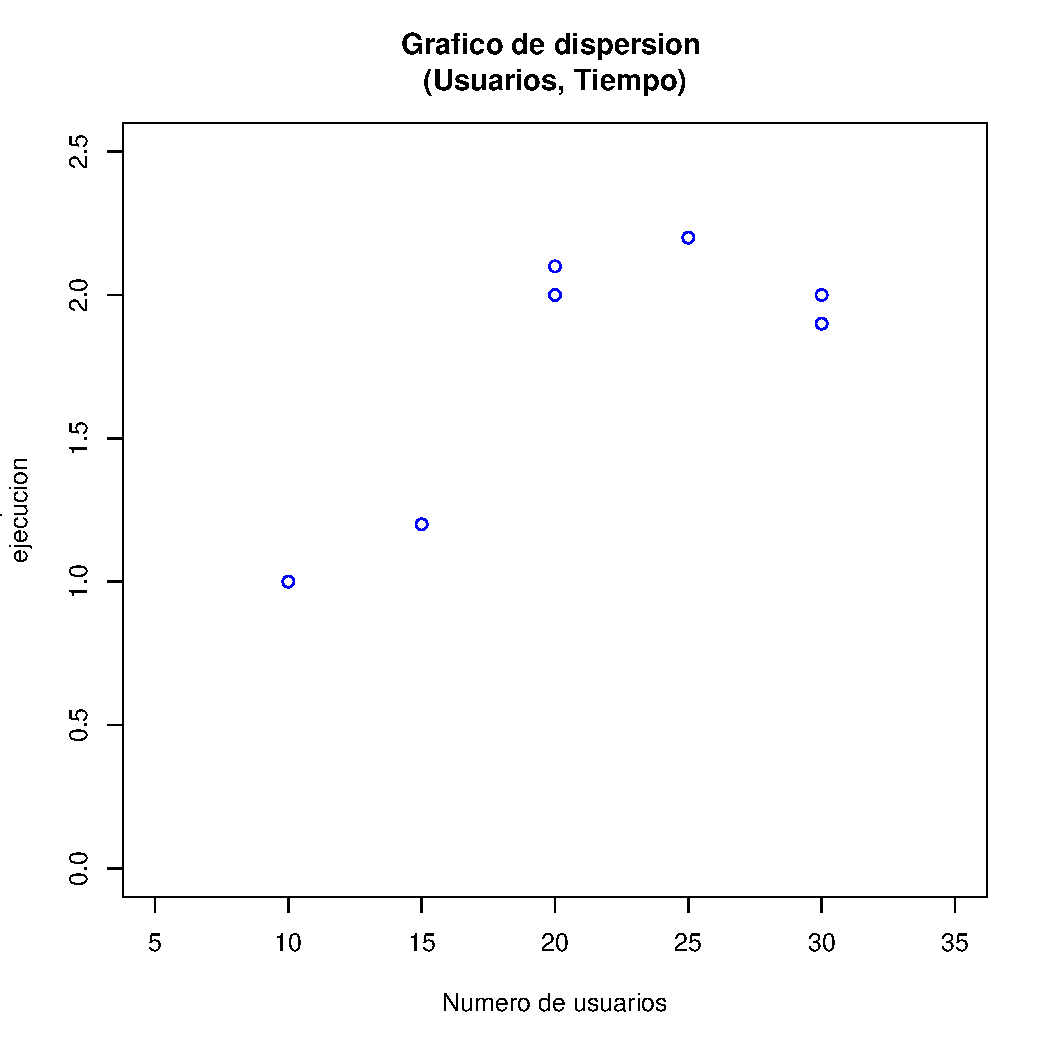
\includegraphics[width=\maxwidth]{figure/unnamed-chunk-9-1} 
\begin{kframe}\begin{alltt}
\hlcom{# Gr\textbackslash{}'afico de pastel (por ser pocos valores)}
\hlkwd{pie}\hlstd{(tfre[[}\hlnum{2}\hlstd{]],} \hlkwc{main}\hlstd{=}\hlstr{"Gr\textbackslash{}'afico de pastel"}\hlstd{,} \hlkwc{xlab}\hlstd{=}\hlstr{"N\textbackslash{}'umero Hijos \textbackslash{}n"}\hlstd{,}
    \hlkwc{col}\hlstd{=}\hlkwd{c}\hlstd{(}\hlstr{"yellow"}\hlstd{,} \hlstr{"blue"}\hlstd{,}\hlstr{"white"}\hlstd{,} \hlstr{"orange"}\hlstd{,} \hlstr{"cyan"}\hlstd{,} \hlstr{"red"}\hlstd{),}
    \hlkwc{sub}\hlstd{=}\hlstr{"Agosto-2012"}\hlstd{)}
\end{alltt}
\end{kframe}
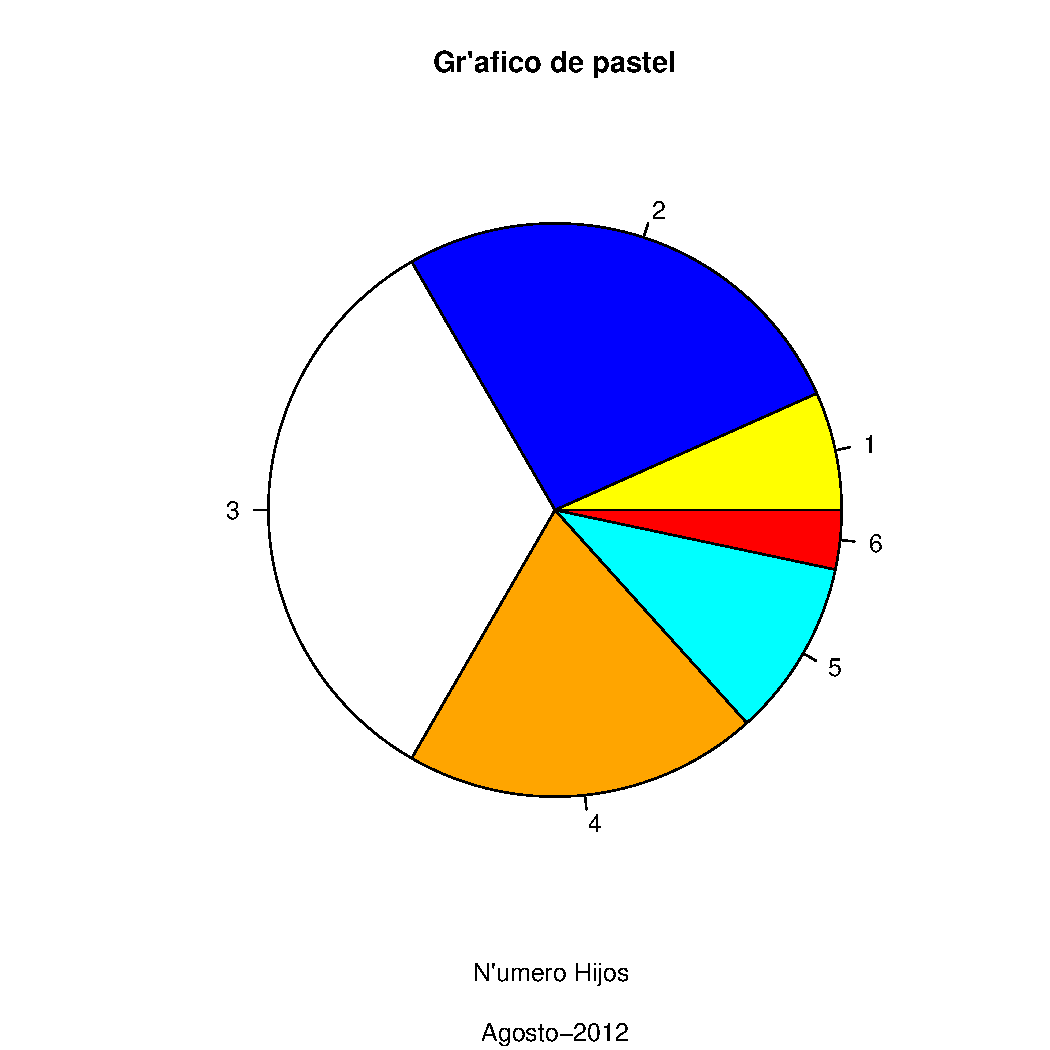
\includegraphics[width=\maxwidth]{figure/unnamed-chunk-9-2} 
\begin{kframe}\begin{alltt}
\hlcom{# Se puede especificar nombres para las categor\textbackslash{}'ias}
\hlkwd{names}\hlstd{(fab)} \hlkwb{=} \hlkwd{c}\hlstd{(}\hlstr{"Cero"}\hlstd{,} \hlstr{"Uno"}\hlstd{,} \hlstr{"Dos"}\hlstd{,} \hlstr{"Tres"}\hlstd{,} \hlstr{"Cuatro"}\hlstd{,} \hlstr{"Cinco"}\hlstd{)}
\hlkwd{pie}\hlstd{(fab,} \hlkwc{main}\hlstd{=}\hlstr{"Gr\textbackslash{}'afico de pastel"}\hlstd{,} \hlkwc{xlab}\hlstd{=}\hlstr{"X = N\textbackslash{}'umero Hijos\textbackslash{}n"}\hlstd{,}
    \hlkwc{col}\hlstd{=}\hlkwd{c}\hlstd{(}\hlstr{"yellow"}\hlstd{,} \hlstr{"blue"}\hlstd{,}\hlstr{"white"}\hlstd{,} \hlstr{"orange"}\hlstd{,} \hlstr{"cyan"}\hlstd{,} \hlstr{"red"}\hlstd{),}
    \hlkwc{sub}\hlstd{=}\hlstr{"Agosto-2012"}\hlstd{)}
\end{alltt}
\end{kframe}
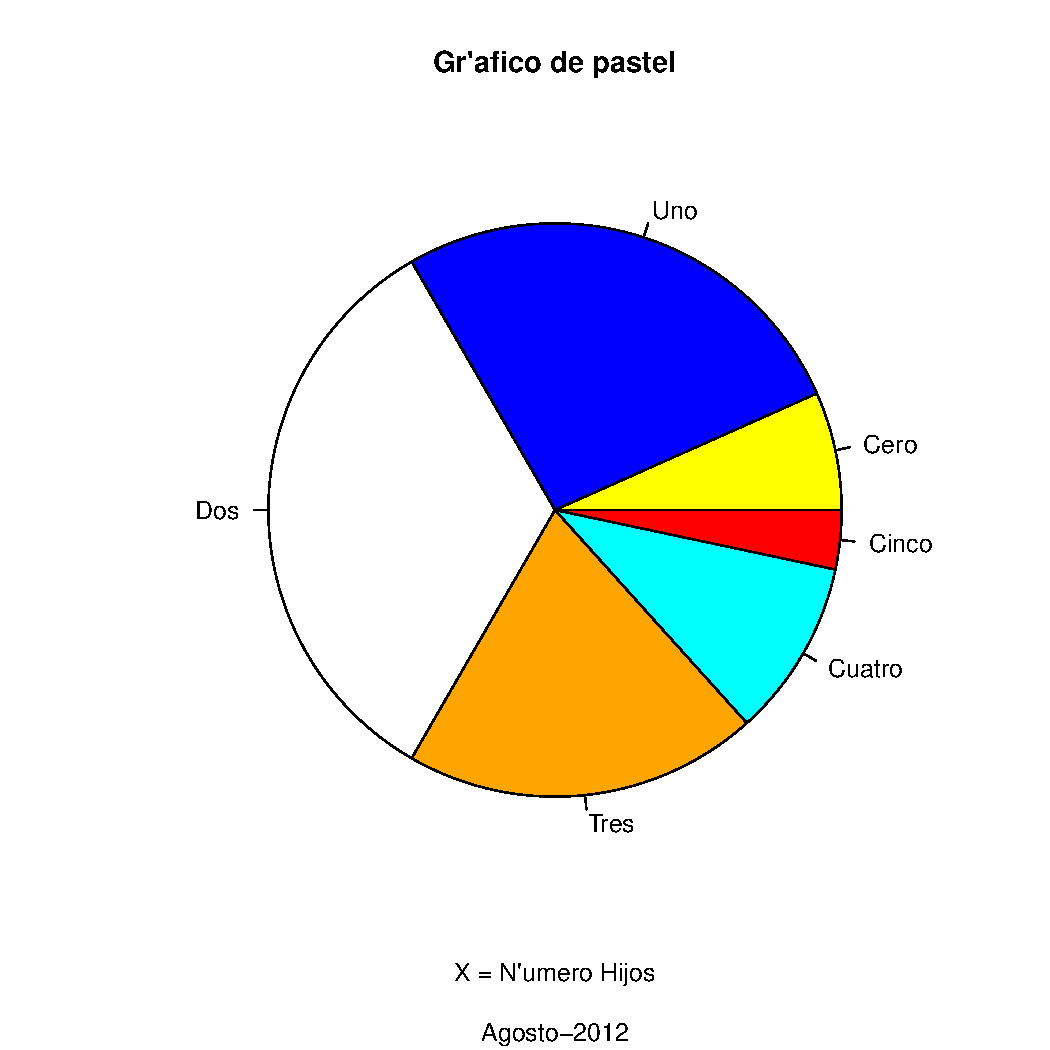
\includegraphics[width=\maxwidth]{figure/unnamed-chunk-9-3} 
\begin{kframe}\begin{alltt}
\hlcom{# Gr\textbackslash{}'afico de cajas (box-plot) es la representaci\textbackslash{}'on gr\textbackslash{}'afica de los cinco n\textbackslash{}'umeros}
\hlcom{# Horizontal}
\hlkwd{boxplot}\hlstd{(X,} \hlkwc{main}\hlstd{=}\hlstr{"Gr\textbackslash{}'afico de caja"}\hlstd{,} \hlkwc{ylab}\hlstd{=}\hlstr{"N\textbackslash{}'umero de hijos\textbackslash{}n"}\hlstd{)}
\end{alltt}
\end{kframe}
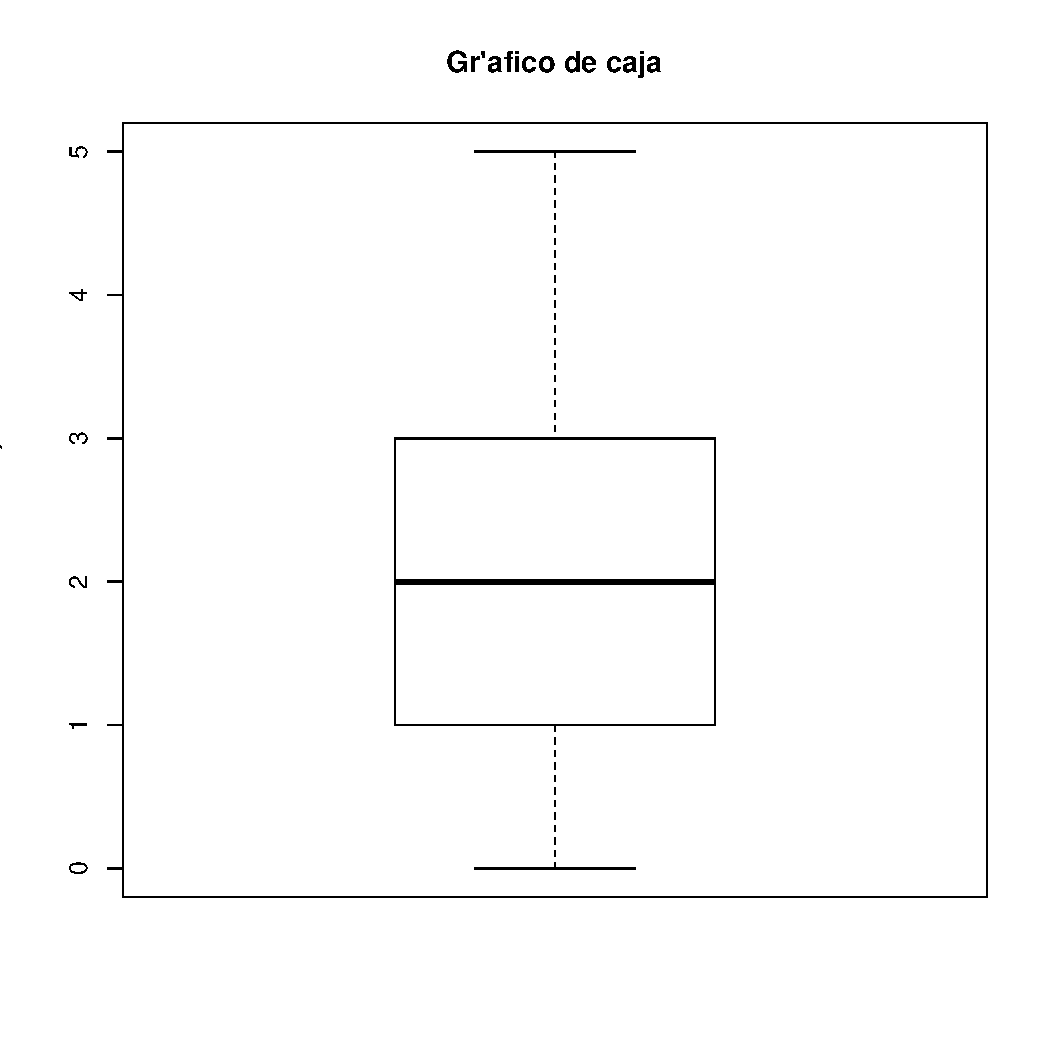
\includegraphics[width=\maxwidth]{figure/unnamed-chunk-9-4} 
\begin{kframe}\begin{alltt}
\hlcom{# Vertical}
\hlkwd{boxplot}\hlstd{(X,} \hlkwc{main}\hlstd{=}\hlstr{"Gr\textbackslash{}'afico de caja"}\hlstd{,} \hlkwc{xlab}\hlstd{=}\hlstr{" N\textbackslash{}'umero de hijos\textbackslash{}n"}\hlstd{,}
        \hlkwc{plot}\hlstd{=}\hlnum{TRUE}\hlstd{,} \hlkwc{border}\hlstd{=}\hlstr{"red"}\hlstd{,}\hlkwc{col}\hlstd{=}\hlstr{"yellow"}\hlstd{,} \hlkwc{horizontal}\hlstd{=}\hlnum{TRUE}\hlstd{)}
\end{alltt}
\end{kframe}
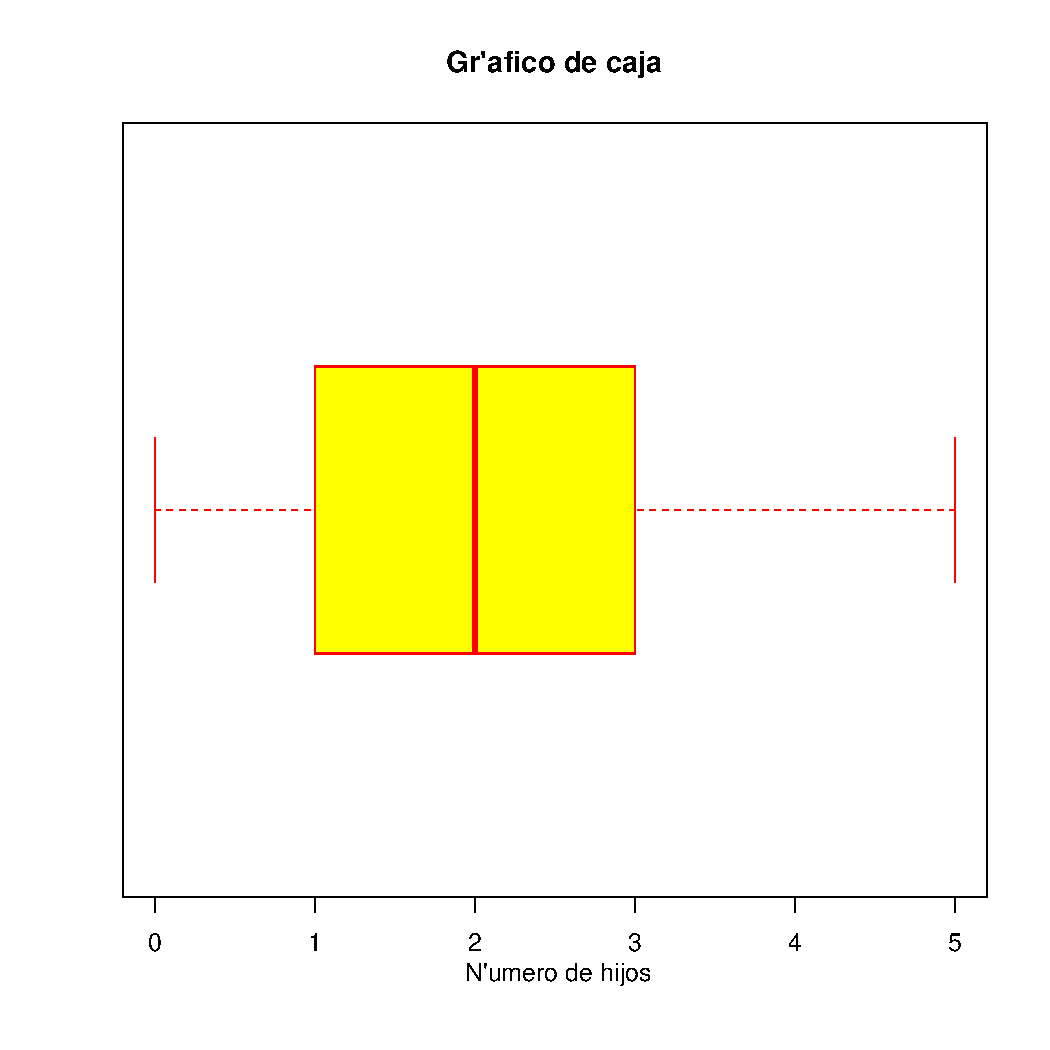
\includegraphics[width=\maxwidth]{figure/unnamed-chunk-9-5} 
\begin{kframe}\begin{alltt}
\hlcom{# NOTE QUE TODOS LOS GR\textbackslash{}'AFICOS DE BARRAS Y DE PASTEL SON REALIZADOS}
\hlcom{# APARTIR DE UNA TABLA DE FRECUENCIA, LA CUAL SE INDICA EN tfre[[2]].}
\hlcom{# TAMBI\textbackslash{}'EN SE PUDO UTILIZAR tabla[[2]].}
\end{alltt}
\end{kframe}
\end{knitrout}
\end{itemize}


\end{document}
